\documentclass[stu,biblatex,floatsintext]{apa7}

\usepackage{graphicx}
\graphicspath{{assets/atwoods-heavy-chain/}}

\usepackage{siunitx}
\usepackage{multirow}

\addbibresource{refs.bib}

\title{Investigating the Effect of Chain Length on Change in Acceleration}
\author{Adam Zhang}
\affiliation{Academies of Loudoun}
\course{AP Physics C: Mech, Block 2}
\professor{Matthew Hilsdorf}
\duedate{September 21 2023}

\begin{document}
\maketitle
\tableofcontents
\newpage

\section{Introduction}

\subsection{Purpose}
Investigate the effect of the length of a heavy chain on the rate of change of the acceleration of the chain as it falls off a pulley.

\subsection{Hypothesis}\label{sec:hypothesis}
An increase in the length of the chain will result in an increase in the rate of change of acceleration of the chain. Since the length of the chain on one side of the pulley is held constant, a longer chain will result in greater weight on one side of the chain, which should increase the rate of change of acceleration as the chain falls.

\subsection{Background}
Atwood's machine is a popular setup to teach basic concepts of motion to physics students. It consists of two weights upon a pulley, as shown in \autoref{fig:atwoods-machine}. When the weight of the string attaching the weights is negligable, the system undergoes constant acceleration in the direction of the heavier weight, $m_1$, according to the below equation \parencite{Zeleny2011AtwoodsMachine}.

\begin{displaymath}
	a = \frac{m_1 - m_2}{m_1 + m_2}g
\end{displaymath}

\begin{figure}[H]
	\centering
	\caption{Basic Setup of Atwood's Machine}
	\label{fig:atwoods-machine}
	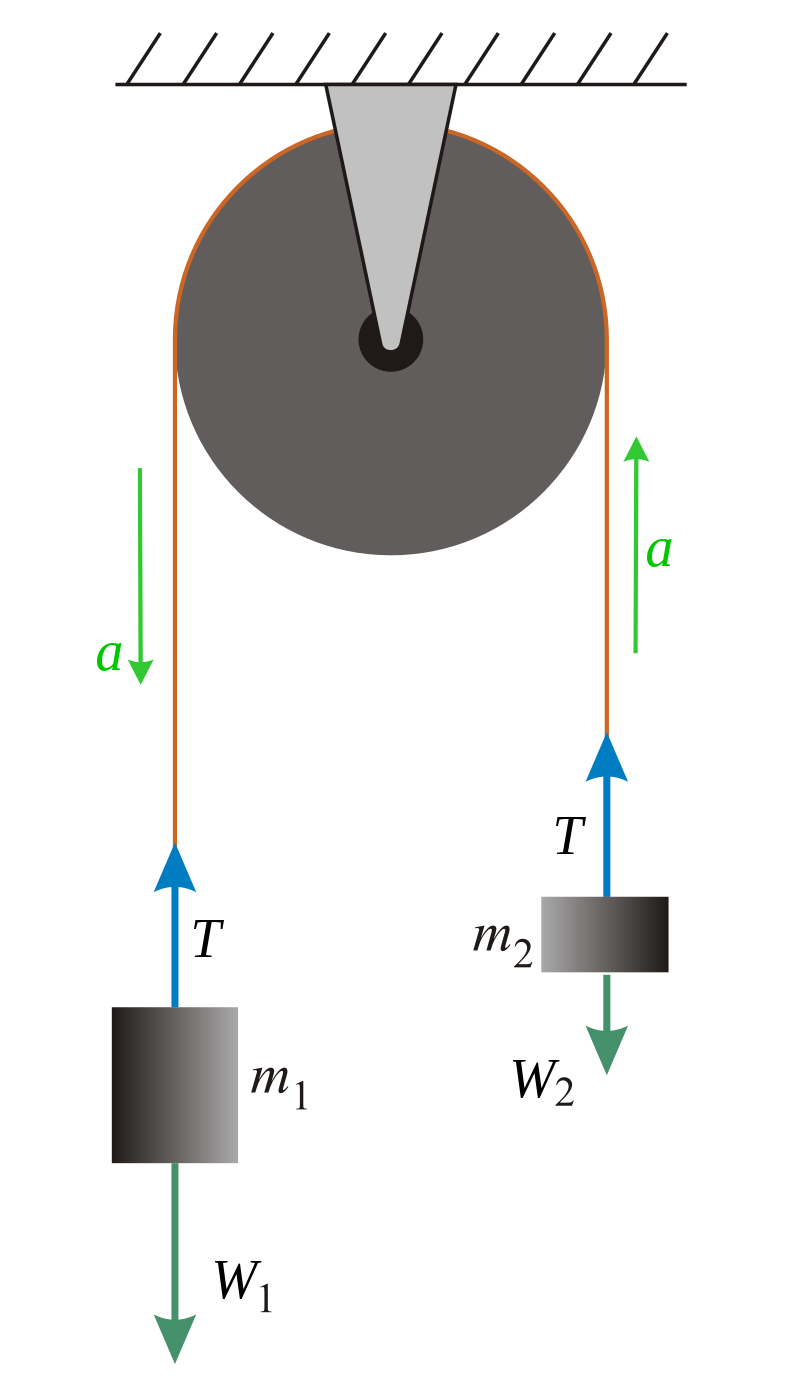
\includegraphics[height=0.25\paperheight]{atwoods-machine-fbd}
\end{figure}

However, one can alter the system of Atwood's machine so that the connecting string's weight is no longer negligible. In this case, the weights attached to the end of the string are no longer necessary, since the weight of the chain itself will cause the motion of the chain falling off of the pulley. The acceleration of this motion is \emph{not} constant. To demonstrate this, \autoref{fig:example-graphs} includes three example graphs of the position, velocity, and acceleration of this motion, from left to right, respectively. As shown, none of the position, velocity, or acceleration versus time graphs exhibit a linear relationship, and the acceleration varies greatly over time \parencite{Hilsdorf2023AtwoodsHeavyChainHandout}. This is the motion that this experiment will investigate.

\begin{figure}[H]
	\centering
	\caption{Example Position, Velocity, and Acceleration Graphs}
	\label{fig:example-graphs}
	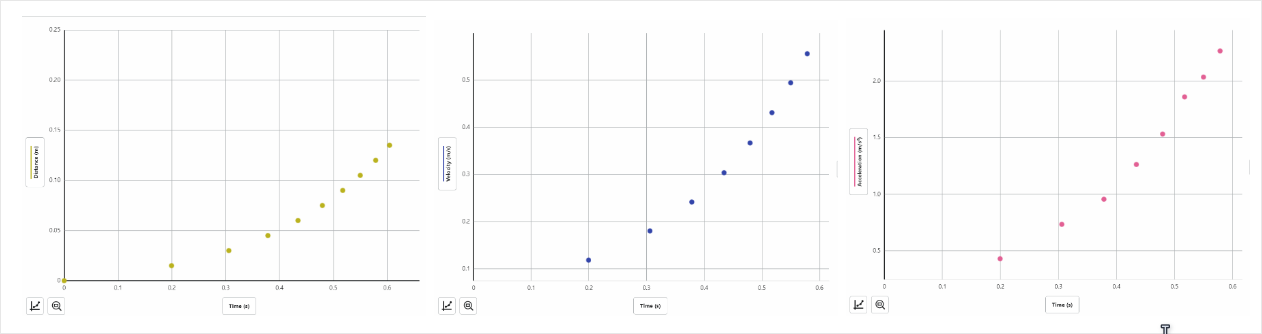
\includegraphics[width=\textwidth]{example-graphs}
\end{figure}

Specifically, this experiment will investigate the relationship between the length of the heavy chain and the rate of change of acceleration. To measure quantitative data, a Vernier photogate will be placed so that it will be able to detect the rotation of the pulley through spokes within the pulley. This photogate will determine the rate of rotation of the pulley, and therefore determine the position of the chain, as well as extrapolate the velocity and acceleration. However, due to the volatility of extrapolated data, extrapolated acceleration will not be used as a quantitative value in this experiment; instead, only the measured velocity will be used.

Given quantative data on velocity, a trend line will be fit to the data to determine an equation that represents the velocity of the chain over time. To determine the acceleration from this equation, the mathematical relationship of the derivative will be used. Calculus defines a derivative as the rate of change of a function; in terms of physics, acceleration can be defined as the rate of change of velocity, and therefore the equation can be determined by taking the derivative of velocity \parencite{Johnson2020VelocityVsAcceleration}.

\section{Methods}

\subsection{Materials}
The following materials are required for this experiment \parencite{Hilsdorf2023AtwoodsHeavyChainHandout}:
\begin{APAitemize}
	\item Vernier ultra pulley (green)
	\item Vernier photogate and connection cable
	\item Vernier LabQuest
	\item Meter stick
	\item 60\unit{\centi\meter}, 70\unit{\centi\meter}, 80\unit{\centi\meter}, 90\unit{\centi\meter}, and 100\unit{\centi\meter} chains\footnote{Note that the chains used in this experiment were not exactly as specified; see \autoref{tab:exact-lengths} for the exact lengths of the chains used.}
\end{APAitemize}
The setup of the experiment is shown in \autoref{fig:setup}.

\subsection{Procedures}
The following procedure was implemented during this experiment.
\begin{APAenumerate}
	\item Construct the experimental setup as shown in Figure \ref{fig:setup}.
	\item\label{pro:outer-start} Place the 60\unit{\centi\meter} chain on the pulley so that 25\unit{\centi\meter} of the chain is on the side away from the photogate.
	\item\label{pro:inner-start} Start collecting data on the LabQuest, then release the chain.
	\item\label{pro:inner-end} End the data collection after the chain has fallen.
	\item\label{pro:outer-end} Repeat steps \ref{pro:inner-start} through \ref{pro:inner-end} two more times to obtain 3 total trials for this length.
	\item Repeat steps \ref{pro:outer-start} through \ref{pro:outer-end} four more times, increasing the chain length by 10\unit{\centi\meter} every time to obtain a total of 15 trials.
\end{APAenumerate}

\begin{figure}[H]
	\centering
	\caption{Experimental Setup}
	\label{fig:setup}
	\includegraphics[height=0.3\paperheight]{setup-diagram}
\end{figure}

\section{Results}

\subsection{Data}
For each trial, a trend line was fitted to the velocity data points. The equation of this velocity line is shown in \autoref{tab:equations}. An example graph for the first trial of the 100\unit{\centi\meter} chain is shown in \autoref{fig:100-trial1}. For completeness, the distance and interpolated acceleration is included in the graph.

\begin{table}
	\centering
	\caption{Trend Line Equations for Each Trial}
	\label{tab:equations}
	\begin{tabular}{|c|c|c|}
		\hline
		Chain Length (\unit{\centi\meter}) & Trial \# & Velocity Equation ($v(t)$) \\
		\hline
		\multirow{3}{*}{60\unit{\centi\meter} Chain}
		& 1 & $0.145e^{5.022t}$ \\
		\cline{2-3}
		& 2 & $0.102e^{5.116t}$ \\
		\cline{2-3}
		& 3 & $0.105e^{5.107t}$ \\
		\hline
		\multirow{3}{*}{70\unit{\centi\meter} Chain}
		& 1 & $0.180e^{5.164t}$ \\
		\cline{2-3}
		& 2 & $0.205e^{5.238t}$ \\
		\cline{2-3}
		& 3 & $0.205e^{5.370t}$ \\
		\hline
		\multirow{3}{*}{80\unit{\centi\meter} Chain}
		& 1 & $0.135e^{5.183t}$ \\
		\cline{2-3}
		& 2 & $0.351e^{4.602t}$ \\
		\cline{2-3}
		& 3 & $0.116e^{5.548t}$ \\
		\hline
		\multirow{3}{*}{90\unit{\centi\meter} Chain}
		& 1 & $0.177e^{5.306t}$ \\
		\cline{2-3}
		& 2 & $0.334e^{5.046t}$ \\
		\cline{2-3}
		& 3 & $0.336e^{5.197t}$ \\
		\hline
		\multirow{3}{*}{100\unit{\centi\meter} Chain}
		& 1 & $0.436e^{4.922t}$ \\
		\cline{2-3}
		& 2 & $0.201e^{5.931t}$ \\
		\cline{2-3}
		& 3 & $0.344e^{5.398t}$ \\
		\hline
	\end{tabular}
\end{table}

\begin{figure}[H]
	\centering
	\caption{Graph for First Trial of 100\unit{\centi\meter} Chain}
	\label{fig:100-trial1}
	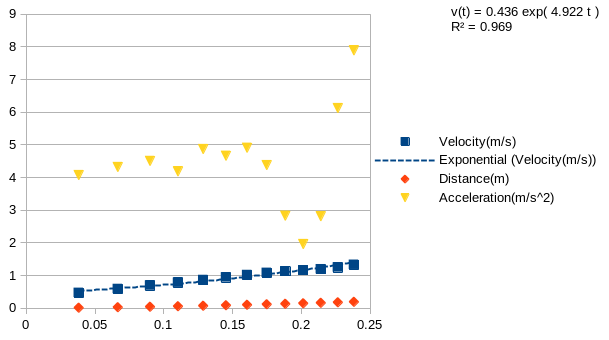
\includegraphics[width=0.75\textwidth]{100-trial1}
\end{figure}

\subsection{Calculations}
The calculated equation for acceleration for each trial is shown in \autoref{tab:acceleration-equation}. The constant for rate of growth for each trial, as well as an average, is shown in \autoref{tab:acceleration-rog}. A scatterplot of the average rate of growth per chain length is shown in \autoref{fig:length-vs-rog}.

\begin{table}
	\centering
	\caption{Equation and Rate of Growth for Acceleration per Trial}
	\label{tab:acceleration-equation}
	\begin{tabular}{|c|c|c|c|}
    	\hline
		Chain Length (\unit{\centi\meter}) & Trial \# & Acceleration Equation ($a(t)$) \\
		\hline
		\multirow{3}{*}{60\unit{\centi\meter} Chain}
		& 1 & $0.728e^{5.022t}$ \\ 
		\cline{2-3}
		& 2 & $0.523e^{5.116t}$ \\
		\cline{2-3}
		& 3 & $2.666e^{5.107t}$ \\
		\hline
		\multirow{3}{*}{70\unit{\centi\meter} Chain}
		& 1 & $0.930e^{5.164t}$ \\
		\cline{2-3}
		& 2 & $1.074e^{5.238t}$ \\
		\cline{2-3}
		& 3 & $1.101e^{5.370t}$ \\
		\hline
		\multirow{3}{*}{80\unit{\centi\meter} Chain}
		& 1 & $0.700e^{5.183t}$ \\
		\cline{2-3}
		& 2 & $1.615e^{4.602t}$ \\
		\cline{2-3}
		& 3 & $0.644e^{5.548t}$ \\
		\hline
		\multirow{3}{*}{90\unit{\centi\meter} Chain}
		& 1 & $0.939e^{5.306t}$ \\
		\cline{2-3}
		& 2 & $1.685e^{5.046t}$ \\
		\cline{2-3}
		& 3 & $1.746e^{5.197t}$ \\
		\hline
		\multirow{3}{*}{100\unit{\centi\meter} Chain}
		& 1 & $2.146e^{4.922t}$ \\
		\cline{2-3}
		& 2 & $1.192e^{5.931t}$ \\
		\cline{2-3}
		& 3 & $1.857e^{5.398t}$ \\
		\hline
    \end{tabular}
\end{table}

\begin{table}[H]
	\centering
	\caption{Rate of Growth of Acceleration}
	\label{tab:acceleration-rog}
	\begin{tabular}{|c|c|c|c|}
    	\hline
		Chain Length (\unit{\centi\meter}) & Trial \# & Rate of Growth & Average \\
		\hline
		\multirow{3}{*}{60\unit{\centi\meter} Chain} & 1 & 5.022 & \multirow{3}{*}{5.082} \\
		\cline{2-3}
		& 2 & 5.116 & \\
		\cline{2-3}
		& 3 & 5.107 & \\
		\hline
		\multirow{3}{*}{70\unit{\centi\meter} Chain} & 1 & 5.164 & \multirow{3}{*}{5.257} \\
		\cline{2-3}
		& 2 & 5.238 & \\
		\cline{2-3}
		& 3 & 5.370 & \\
		\hline
		\multirow{3}{*}{80\unit{\centi\meter} Chain} & 1 & 5.183 & \multirow{3}{*}{5.111} \\
		\cline{2-3}
		& 2 & 4.602 & \\
		\cline{2-3}
		& 3 & 5.548 & \\
		\hline
		\multirow{3}{*}{90\unit{\centi\meter} Chain} & 1 & 5.306 & \multirow{3}{*}{5.183} \\
		\cline{2-3}
		& 2 & 5.046 & \\
		\cline{2-3}
		& 3 & 5.197 & \\
		\hline
		\multirow{3}{*}{100\unit{\centi\meter} Chain} & 1 & 4.922 & \multirow{3}{*}{5.417} \\
		\cline{2-3}
		& 2 & 5.931 & \\
		\cline{2-3}
		& 3 & 5.398 & \\
		\hline
    \end{tabular}
\end{table}

\begin{figure}[H]
	\centering
	\caption{Chain Length vs Average Rate of Change}
	\label{fig:length-vs-rog}
	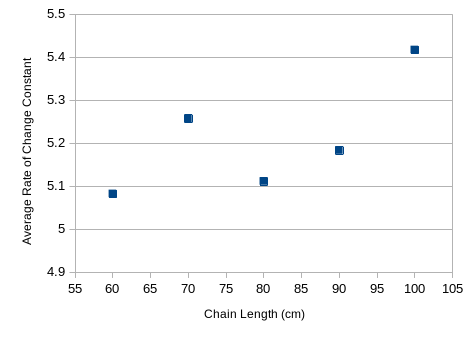
\includegraphics[width=0.75\textwidth]{chain-length-vs-rog}
\end{figure}

\section{Discussion}

\subsection{Conclusion}
The success of the experiment is questionable, since the existence of a relationship between chain length and rate of change of acceleration, such as the \hyperref[sec:hypothesis]{hypothesis}, cannot be confirmed nor rejected. As shown in \autoref{tab:acceleration-rog} and \autoref{fig:length-vs-rog}, there is a generally positive correlation between chain length and the rate of change constant of acceleration. However, the data point for the chain length of 70\unit{\centi\meter} does not fit that trend. Therefore, no conclusive claim can be made. The lack of conclusive evidence likely results from the \hyperref[sec:errors]{many errors} in this experiment.

\subsection{Errors}\label{sec:errors}
There were many potential sources of error in this lab, both physical and procedural. Since the chain was placed upon the pulley and released by hand, it is impossible to guarantee that 25\unit{\centi\meter} of the chain was placed on one side with any amount of acceptable precision. Additionally, initial acceleration may have been added to the pulley system when releasing the chain.

The small number of pruned data points is also a concerning area of error. While multiple trials were performed to attempt to offset this shortcoming, due to the quick nature of the motion being measured, the number of data points collected per trial were relatively small. Additionally, since data was pruned by hand, some data may have been incorrectly cleaned or handled, or may have been subject to selection bias.

Many measures could be taken to increase robustness of similar experiments in the future. More reproducible pulley setups should be used to ensure that the length of chain hanging off one side of the pulley can be measured to a reasonably precise amount. Additionally, more advanced software techniques should be employed to ensure that the calculation and analysis of data is more accurately representative of the actual motion.

\subsection{Extensions}
Systems of pulleys are extensively used in many areas of modern technology, such as elevators, construction, and exercise machines \parencite{Vork2018PulleyExamples}. Understanding the underlying mechanics in the motion of pulleys is essential in utilizing them correctly and safely to their full potential.

\printbibliography

\appendix

\section{Tables}

\begin{table}
	\centering
	\caption{Exact Lengths of Chains Used}
	\label{tab:exact-lengths}
	\begin{tabular}{|c|c|}
		\hline
    	Colloquial Length (\unit{\centi\meter}) & Exact Length (\unit{\centi\meter}) \\
		\hline
		60 & 59.0 \\
		\hline
		70 & 69.4 \\
		\hline
		80 & 80.0 \\
		\hline
		90 & 89.5 \\
		\hline
		100 & 99.6 \\
		\hline
    \end{tabular}
\end{table}

\end{document}
